\documentclass{report}


\usepackage{bibgerm}
\usepackage[numbers,sort&compress]{natbib}
\usepackage{amsmath,amssymb,mathtools}
\usepackage{algpseudocode,algorithm}
\usepackage{graphicx}
\usepackage{hyperref}
\usepackage{multirow}
\usepackage[utf8]{inputenc}
\usepackage{geometry}
\usepackage{parskip}
\usepackage{paralist}

\geometry{verbose,a4paper,tmargin=25mm,bmargin=25mm,lmargin=15mm,rmargin=20mm}

%% Stuff ist aus ML1. vllt brauchen wir es ja noch :D
\DeclareMathOperator*{\argmax}{arg\,max}
\DeclareMathOperator*{\argmin}{arg\,min}

\newcommand{\IndState}[1][1]{\State\hspace{10mm}}
\newcommand{\mparagraph}[1]{\paragraph{#1} \mbox{}\\}

%%%%%%%%%%%%%% includeonly %%%%%%%%%%%%%%%%%%%
% Es werden nur die Teile eingebunden, die hier
% aufgefuehrt sind!
%\include{Kapitel X}
%}um es anzuzeigen.
%%%%%%%%%%%%%%%%%%%%%%%%%%%%%%%%%%%%%%%%%%%%%%
\graphicspath{{pic/}}

\begin{document}
\tableofcontents

% einfach !TEX root = swt2.tex an den Anfang packen von chaptern
% !TEX root = swt2.tex
\chapter{Software Development Process}

\section{Code and Fix}
Drauf los programmieren, sehen obs funktioniert. Wenn nicht wird es geändert,
so dass es funktioniert. \\

\textbf{Probleme:}
\begin{compactitem}
    \item Schlecht strukturierter Code (keine Planung im Voraus)
    \item Nicht systematische Verbesserungen
    \item Schwer im Team umzusetzen, da keine Einteilung existiert
    \item Kein Entwurf oder Dokumentation
    \item Wartbarkeit sehr schwierig (schlechte Doku, keine Struktur)
\end{compactitem}

\section{Prozessmodell}
Ein Prozessmodell (''Vorgehensmodell'') ist eine abstrakte Repräsentation
des Software Entwicklungsprozesses. Beschreibt den Prozess aus einer bestimmten
Perspektive.\\

\textbf{Richtlinien:}
\begin{compactitem}
    \item Welche Aktivitäten sollen ausgeführt werden (Wann? In welcher
    Reihenfolge?)
    \item Wer macht was? Rollen und Verantwortlichkeiten
    \item Welche Produkte (Artefakte, Code, Dokumente) sollen bis wann erstellt
    werden
    \item Manchmal welche Techniken und Werkzeuge verwendet werden.
\end{compactitem}
\subsection{Vorteil von Prozessmodellen}
\begin{compactitem}
    \item Klardefinierte Arbeitspakete/Aufgaben $\Rightarrow$ Bessere Verteilung
    auf Team
    \item Fortschritt feststellbar ('' Wo stehe ich in meinem Projekt '')
    \item Verbesserung der Wartbarkeit (Dokumentation)
    \item Geringeres Projektrisiko
    \item Höhere Produktqualität
    \item Explizite Phase der Qualitätssicherung
\end{compactitem}
Vorteile hängen jedoch vom konkreten Projekt und den gewählten Prozessen ab.


\section{Shitty Models}
\begin{compactitem}
    \item Wasserfallmodell
    \item V-Modell
    \item Spiralmodell (Kombination Wasserfall + V Modell)
\end{compactitem}
Können als Blöcke für Software Entwicklungs Prozesse gesehen werden.

\section{Unified Process, UP}
\subsection{Phases}
\begin{compactitem}
    \item Inception (Anfangsphase): Projektumfang klarmachen, Vision und Business
    Case
    \item Elaboration (Ausarbeitungsphase): Hauptarchitektur bauen, Elemente mit
    hohem Risiko lösen, meisten Anforderungen festlegen, allgemeinen Zeitplan
    schätzen
    \item Construktion (Konstruktionsphase): inkrementelle Implementierung der
    restlichen Elemente mit geringerem Risiko
    \item Transition (Übergabephase): Beta Tests, deployment
\end{compactitem}
\subsection{Disciplines}
\begin{compactitem}
    \item Business modelling: Verstehen und Kommunizieren der Struktur der Organisation
    wo das System verwendet wird.
    \item Requirements
    \item Design
    \item Implementation
    \item Test
    \item Deployment
\end{compactitem}
\section{Rational Unified Process RUP}
Bestimmte Implementierung des UP. Zustätzlch zu Phasen und Disciples gibt es:
\begin{compactitem}
    \item Rollen, wer macht was?
    \item Activities/Tasks, wie wird es gemacht?
    \item Artifacts/work products, was wird gemacht?
\end{compactitem}

\subsection{Best Practices}
\begin{compactitem}
    \item software iterativ entwickeln
    \item Anforderungen managen
    \item component-basierte Architekturen verwenden
    \item Software visuell modellieren
    \item Software auf qualität testen
    \item Kontrolle wird zu Software
\end{compactitem}

% !TEX root = swt2.tex
\chapter{Agile Development}

\section{Agile Manifesto}

Rechts ist wichtig, aber links ist wichtiger!
\begin{compactitem}
    \item Individuals and Interaction $\xrightarrow{\text{over}}$ Process and Tools
    \item Working Software $\xrightarrow{\text{over}}$ Comprehensive documentation
    \item Customer collaboration $\xrightarrow{\text{over}}$ contract negotiations
    \item Responding to change $\xrightarrow{\text{over}}$ Following a plan
\end{compactitem}

\section{Extreme Programming}

\subsection{Values}
\begin{compactitem}
    \item Communication
    \item Simplicity
    \item Feedback
    \item Courage
\end{compactitem}
\subsection{Some Principles}
\begin{compactitem}
    \item Quick delivery
    \item rapid feedback
    \item keep it simple
    \item incremental change
    \item embrace change
\end{compactitem}

\chapter{Requirements Engineering}


\section{Requirements Elicitation Technique}
\begin{itemize}
    \item Questioning techniques
    \item Creativity techniques (Brainstorming, Analogy, Perspektivenwechsel)
    \item Retrospective techniques (Reuse, System archeology, competing systems)
    \item Observation techniques
    \item Supporting actions and techniques (Mind Maps, Workshops, User Stories,
    Use Case modelling etc...)
\end{itemize}

\section{Concerned Based Classification / Bedürfnisbasiert}
Schwer funktionale und nicht-funktionale Anforderungen zu definieren, da sehr
schwammig. Daher Anforderungen lieber basierend auf zugrunde liegendm Bedürfniss.
\begin{itemize}
    \item Representation
    \begin{itemize}
        \item Operational
        \item Quantitative
        \item Qualitative: Nicht direkt verifizierbar
        \item Deklarative
    \end{itemize}
    \item Kind
    \begin{itemize}
        \item Functional
        \item Quality
        \item Constraint
    \end{itemize}
\end{itemize}


\section{Basic Writing Recommendation}
\begin{itemize}
    \item Kurze Sätze, Ein Requirement pro Satz
    \item Aktive Sprache, wer macht was
    \item ,,Schwache'' Wörter vermeiden
    \item Glossar an Worten/Termen bereit haben
\end{itemize}

\section{Requirement Validation Techniques}
\begin{itemize}
    \item Inspection, Reviews, Walkthroughs: finde Fehler manuell
    \item Simulation: Aspekte des Systems simulieren.
    \item Prototyping: orienterit a design. Stakeholder testet Szenarien im
    Prototyp
    \item Creation of system test cases
    \item Model Checking: formale Verifikatio des verwendeten Models
\end{itemize}

\chapter{Use Cases}

% !TEX root = swt2.tex

\chapter{Model Driven Development}

\section{Ziele und Vorteile}
\mparagraph{Ziele}
\begin{compactitem}
    \item Bessere Platform Unabhängigkeit und Kompatibilität
    \item Schnelleres Entwickeln durch Code Generierung
    \item Bessere Software qualität durch vorherige Analysen
    \item Besserer Wiederverwendung
    \item Besserer ,,Separation of concers'' durch verschiedener Modelle
    \item Komplexität nicht verringern, sondern auf einem anderne Level zu
    managen durch Abstraktion
\end{compactitem}
\mparagraph{(erhoffte) Vorteile}
\begin{compactitem}
    \item Kostenreduzierung
    \item Kürzere time to market
    \item Mehr Variabilität
\end{compactitem}

\section{Arbeiteraufteilung bei MDSD}
\begin{compactitem}
    \item \textbf{Programmer}: Nicht mehr notwendig
    \item \textbf{Domain Expert}: Entwickelt Software. Weiss wie Problem aussieht,
    was rauskommt, was zu tun ist.
    \item \textbf{Technology Expert}: Liefert Methoden und Tooling damit Domain
    Expert arbeiten kann. Überlegung von Meta Modellen, Modellierung der Plattform
    und Transformationen
\end{compactitem}

\section{Warum Modelle?}
\begin{compactitem}
    \item Verringern Komplexität bzw. Fokus auf das Wesentliche
    \item erhöht Analysierbarkeit
    \item Besser mit Komplexität umgehen
    \item Verwendbar vom Domain Expert
    \item Erhöhte Kommunikation
    \item evtl eine immer konsistene Dokumentation
\end{compactitem}

\section{Definition Modell}
Eine formale Repräsentation einer
Wiedergabe eines Originals (natürlich oder künstlich) mit dessen Attributen und
Beziehungen (Reproduction). \\
Es werden nicht alle Attribute verwendet, nur die relevanten (Abstraktion).
Wird für einen bestimten Zweck verwendet (wer, wann und wozu benutzt werden?)
(Pragmatik)

\section{Meta Modell}
Ein Meta-Modell ist ein Modell, das die Elemnte  und Beziehungen einer
Modellierungssprache sowie Einschränkungen und Regeln wie valide Modelle erstellt
werden beschreibt. Umfasst
\begin{compactitem}
    \item \textbf{Abstrakte Syntax}: Was sind die Elemente und was sind die Beziehungen.
    \item \textbf{Konkrete Syntax}: Repräsentation. Wie schreibe ich etwas hin.
    \item \textbf{Statische Semantik}: Prüfung vor konkreter Modellinstanz möglich.
    Was muss für jede Modllinstanz gelten.
    \item \textbf{Dynamische Semantik}: Was drückt das Meta ;odell aus?
\end{compactitem}

\section{Object Constraint Language}
Ausdruck von Einschränkungen und Regeln von Meta Modellen.
Genaue Spezifikationen in Transformationen nutzen.
Eine beschreibende Sprache, welche folgende Spezifikationen erlaubt:
\begin{compactitem}
    \item Invarianten
    \item Vor und Nachbedingungen
    \item Initialwerte
    \item Ableitungen
    \item Body Definitions
    \item Guards
\end{compactitem}

\chapter{Analysis}

\chapter{Software Architecture}

% !TEX root = swt2.tex
\chapter{Software Components}

Eine Komponente ist ein Baustein, der zusammengesetzt, angepasst und
eingesetzt werden, ohne sein inneres zu kennen.
Modularer Austauschbarer Teil eines Systems. \\

Ein Java Objekt kann keine Komponente sein, da das Black-Block Prinzip
bei der Vererbung verletzt wird.

\section{Component Modell}
Ein Komponentenmodell definiert:
\begin{compactitem}
    \item Was ist eine Komponenten?
    \item Wie bietet diese Komponente ihre Dienste an?
    \item Wie sind Komponenten verbunden und zusammengesetzt?
    \item Wie kommunizieren Komponenten?
    \item Wo findet man Komponenten?
\end{compactitem}

\section{Service Oriented Architecture, SOA}
Elemente aus einem Web Service System haben eine von 3 Rollen:
\begin{compactitem}
    \item Service Provider
    \item Service Broker
    \item Service Requestor
\end{compactitem}

\section{Palladio Component Model}
Ist eine Domain Spezifische Modellierungs Sprache (DSL) zur frühzeitigen
Performancevorhersagen.

\subsection{Komponentenbeschreibung, Modelle und Entwickler}
\begin{itemize}
    \item \textbf{Komponenten/Component Model}: Code der Komponenten
    \begin{compactitem}
        \item \textbf{Komponententwickler} spezifiziert und entwickelt Komponenten
        \item ... Spezifiziert Datentypen
        \item ... Baut zusammengesetzte Komponenten
        \item ... Baut parametrisierte Komponenten
        \item ... Lagert Moddeling und Implementierungs Artefakte in Repositorys
    \end{compactitem}
    \item \textbf{Komposition/Composition Model}: Verschaltung/Vernetzung verschiedene  Komponenten
    \begin{compactitem}
        \item \textbf{Softwarearchitekt}: Spezifiziert eine Architektur (System Modell)
        \item ... spezifiziert neue Komopnenten und Schnittstellen.
        \item ... Benutzt Architekturstyles und Patterns
        \item ... trifft Design Entscheidungen
        \item ... macht Performancevorhersagen
        \item ... delegiert Implementierung
        \item ... leitet den gesamten Entwicklungsprozess
    \end{compactitem}
    \item \textbf{Resourcen Environment/Deployment Model}: Hardware
    \begin{compactitem}
        \item \textbf{System Deployer}: Modelliert Resourcenumgebung (Middleware, OS, Hardware...)
        \item ... Modelliert die Allokation von Komopnenten zu Resourcen
        \item ...Wartet das System
        \item ... Richtet Resourcenumgebung ein
        \item ... Deployed Komponenten
    \end{compactitem}
    \item \textbf{Usage Profile/Usage Model}: Wieviel Benutzer? Wieviel Daten?
    Welche Daten? etc.
    \begin{compactitem}
        \item \textbf{Domain Expert}: kennt sich mit der business domain aus.
        \item ... spezifiziert Nutzerverhalten.
    \end{compactitem}
\end{itemize}

Mit den Einflussfaktoren lässt sich die Antwortzeit, die Resourcennutzung und der
Durchsatz berechnen.

\subsection{Vorteile}
\begin{compactitem}
    \item Erweiterung von Legacy Software Systemen
    \item Performancevorhersagen
    \item Analytisch lösbar
    \item Simlation
\end{compactitem}

\subsection{Sichten in Palladio}
\begin{compactitem}
    \item \textbf{Strukturel}: Informationen über statische Eigenschaften des Systems.
    Wird vom Component Developer und Softwarearchitekt modelliert. (component view, assembly view)
    \item \textbf{Verhalten}: Ablaufdiagramme von Verhalten. Wird vom Component
    Developer (und Softwarearchitekt) modelliert. (intra und inter component, behaviour )
    \item \textbf{Deployment}: Information wie wird System eingesetzt wird.
    Modelliert vom System Entwickler (allocation)
    \item \textbf{Decision}: Wird durch alle 3 Rollen modelliert
\end{compactitem}

\subsection{Service Effect Specification, SEFF}
\begin{compactitem}
        \item Beschreibt die externen sichtbaren Aktionen eines Komponente erbrachten Diensts.
        \item Abstraktion interner Verhalten
        \item Beschreibt Zusammenhang zwischen bietender und benötigender Komponentenseite
        \item Parametrisierung von Resourcenverbrauch
\end{compactitem}

\chapter{Patterns of Enterprise Application Architecture}

Softwareanwendungen, die zu Unternehmenszwecken verwendet werden.

\mparagraph{Eigenschaften}
\begin{compactitem}
    \item Bestenhende Daten. Langlebiger als Anwendung und Hardware
    \item Große Datenmengen.
    \item Gleichzeitiger Zugriff auf die Daten
    \item Schnittstelle zu anderen Systemen
    \item Unterschiedliche Nutzer (erfahren, unerfahren)
    \item Geschäftsregeln und Prozesse sind komplex, aber nicht unbedingt logisch.
\end{compactitem}

\section{Schichten von EA}
\begin{compactitem}
    \item \textbf{Präsentation}: Interaktion von User und Software handhaben. Informationen darstellen und
    Eingaben interpretieren.
    \item \textbf{Domäne}: Datenverarbeitung
    \item \textbf{Data Source}: Kommunikation mit anderen Systemen. Datenbanken etc.
\end{compactitem}

\section{EA Patterns}

\subsection{Domain Logic Patterns}
Wie am besten Geschäftsregeln repräsentieren?
Umsetzung von Geschäftslogik
\subsubsection{Transaction Script}
Organisiere Geschäftslogik in einzelne Prozeduren. Jede Prozedur bearbeitet eine einzelne
Anfrage der Presentationsschicht.
Pro Aufgabe implementiere eine Methode.

+ Einfach \\
+ einfach zu verbinden mit anderen Datenquellen \\
+ Transaktionsgrenzen leicht zu bestimmen. \\
- Skaliert nicht gut mit komplexerer Domänenlogik \\
- Code muss evtl. dupliziert werden

\subsubsection{Domain Model}
Strukturiere Domänenlogik anhand eines Objektmodells sodass Objekte sowohl Verhalten als auch Daten
enthalten. Objekte arbeiten zusammen um Transaktion durchzuführen.

+ Besser bei komplexeren Logik \\
- Verbindung mit Datenquelle komplexer
- Flachere Lernkurve wenn nicht vertraut mit OO ist.

\subsubsection{Table Module}
Einzelne Instanz einer Klasse behandelt die Geschäftslogik für alle Reihen/Zeilen
einer Tabelle oder Views. Pro Tabelle eine Klasse.

+ direktes Mapping auf Daten \\
+ Separiert Logik für verschiedene Konzepte \\
- Keine Objekt Instanzen: kann schlecht für komplexere Logik sein.

\begin{figure}[!h]
    \centering
    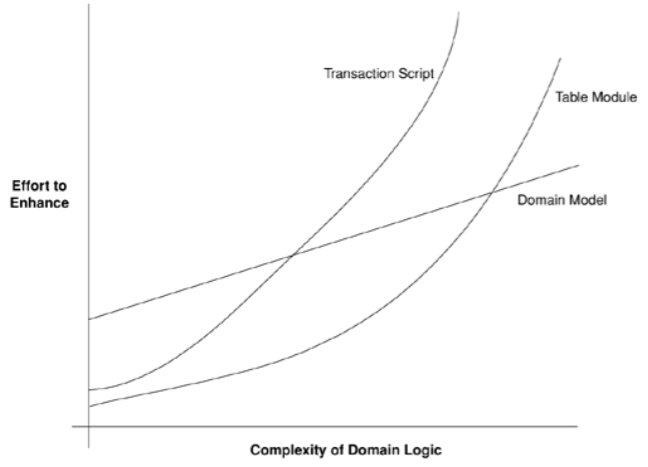
\includegraphics[scale=0.5]{domainlogik}
\end{figure}

\subsection{Data Source Architecture}
Wie Domänen Logik und Datenquelle separieren?
\subsubsection{Record Set}
In-Memory Repräsentation der Daten. Direktes Ergebnis einer SQL-Query

\subsubsection{Table Data Gateway}
Ein Objekt, dass als Gateway zu einer Datenbanktabelle fungiert. Eine Instanz des Table Data Gateway
behandelt alle Reihen der Tabelle. Instaz behinahltet notwendiges SQL für Interaktion mit
kompletter Tabelle.
Trennung von SQL Statements und Code der zugriff auf Daten hat.

Unterschied Facade und Gateway: Spezielle Nutzen vs. allgemeiner Nutzen (facade)

\subsubsection{Active Record}
Ein Objekt, dass eine Reihe aus einer Datenbanktabelle oder View wrapped.
Kapselt Datenbank Zugriff und kann Domänenlogik auf den Daten ausfühen.
Bringt Daten und Funktionalität zusammen.

+ Gut bei sehr einfacher Domänenlogik
- Datenbankschema und Active Record müssen Isomorph sein (1:1 mapping). Schwierigkeiten für
komplexere Logik mit Vererbung

\subsubsection{Row Data Gateway}
Ein Objekt, dient als Gateway eines einzelnen Datensatzes/Zeile einer Datenbank. Eine Instanz pro
Zeile.

Trennung von Datenbank Zugriff und Objekte im Speicher.

\subsubsection{Data Mapper}
Mapper, der Objekte im Speicher auf Datenbank abbilden kann. Beides bleibt komplett unabhängig.
Trennt Datenbank-Logik und Domänenlogik

\subsection{when to use what?}
\begin{compactitem}
    \item \textbf{Transaction Script}:
    \begin{compactitem}
        \item Row Data Gateway: Explizite Schnittstelle, besser weiter zu entwickeln
        \item Table Date Gateway: Wenn Record Set Framework
    \end{compactitem}
    \item \textbf{Domain Model}
    \begin{compactitem}
        \item Simpel: Active Record
        \item Komplexes Mapping: Data Mapper
    \end{compactitem}
    \item \textbf{Table Module} (Wenn Record Set Framework)
    \begin{compactitem}
        \item Table Data Gateway
    \end{compactitem}
\end{compactitem}
\subsection{Object-relational structural pattern}
Wie Objekte auf relationale Datenbank abbilden?
Alle Patterns sind für Domänenmodells mit Data Mapper gedacht.
\subsubsection{Single Table Inheritance}
Repräsentiert Vererbungshierarcie der Klassen als eine einzelne Tabelle welche Spalten mit allen
Feldern der verschiedenen Klassen hat.

+ Komplette Hierarchie in einer Tabelle\\
+ Keine Joins nötig \\
- Verschwendeter Platz für Spalten\\
- Zugriff ist Bottleneck

\subsubsection{Class Table Inheritance}
Eine Tabelle pro Klasse. Attribute sind verteilt

+ Klare Struktur \\
- Schlechte performance
- Benötigt Joins
\subsubsection{Concrete Table Inheritance}
Eine Tabelle pro konkrete Klasse mit allen Attributen.
+ keine Joins nötigt \\
- Finden erfordert mehrere Queries \\
- Änderungen der Superklasse beeinflusst alle anderen Tabellen.

% !TEX root = swt2.tex
\chapter{Software Design}
Design Class Diagrams müssen Definitionen der Software Klassen zeigen.

\section{Responsibility-Driven Design}

Softwareobjekte sind ähnlich zu Echtwelt Objekten. Daher ist wichtige Aufgabe Software Objekten
Verantwortungen zuzuweisen. Verantwortung ist abhängig von seinem Verhalten.
\begin{compactitem}
    \item doing responsibilities: doing something itself, controlling and coordinating activities
    in other objects
    \item knowing responsibilities: knowing about private encapsulated data, knowing about related
    objects, knowing about things it can derive or calculate
\end{compactitem}

\mparagraph{Zuweisung}
Verwende Operation Contracts der System Operationen. Nutze diese zum finden von Interaktionen zwischen
Objekten.

\section{Dynamic und Static Design Model}

Startpunkt eines Design Class Diagrams.
Interaktion zwischen einzelne Objekten modellieren. Wo weise ich Verantwortungen zu?
\mparagraph{Identifizieren}
\begin{compactenum}
    \item Klassen, die in der Softwarelösung teilnehmen
    \item Zeichen Klassendiagramm dieser lassen
    \item Identifiziere Klassenmethoden durch Analyze des Interaktionsdiagramm
\end{compactenum}

Static Design Model aus Dynamic Design Model Schritt für Schritt ableitbar.

\section{General Responsibility Assignment Software Patterns, GRASP}

Abgesehen von dem Fakt, dass man ywischen Domäne und Softwareobjekten eine geringe Repräsentationsdistanz
haben möchte (Design Konzept lässt sich nahtlos vom Domänen Konzept ableiten), will man wissen,
wie man Interaktions Diagramme systematisch erstellt.
\begin{compactenum}
    \item Informations Experte
    \item Creator: Welches Objekt ist dafür zuständig X zu erzeugen?
    \item Controller: Verantwortung für Empfangen und Handhaben von System Event Nachrichten
    \item Low coupling : Versuche eine geringe Verkoppelung im System zu haben.
    \item High Cohesion
    \item Polymorphism: Composition statt Inheritance
    \item Pure Fabrication: Künstliche Klasse erfinden, wenn Domänen objekt nicht existiert.
    \item Indirection: Adapterobjekt als Mediator zwischen Objekten falls Verantwortungszuweisung zu
    high coupling oder low cohesion führt.
    \item Protected Variations: informationen verstekcen.

\end{compactenum}

\chapter{Clean Code}

\chapter{Real-time Development & Patterns}

\include{13_reliability}
\chapter{Software Security}

\chapter{Continuous Integration}



\end{document}
